\documentclass[11pt]{article}
\usepackage[UTF8]{ctex}
\usepackage[a4paper]{geometry}
\geometry{left=2.0cm,right=2.0cm,top=2.5cm,bottom=2.5cm}

\usepackage{comment}
\usepackage{booktabs}
\usepackage{graphicx}
\usepackage{diagbox}
\usepackage{amsmath,amsfonts,graphicx,amssymb,bm,amsthm}
\usepackage{algorithm,algorithmicx}
\usepackage[noend]{algpseudocode}
\usepackage{fancyhdr}
\usepackage{tikz}
\usepackage{graphicx}
\usepackage{verbatim}
\usetikzlibrary{arrows,automata}
\usepackage{hyperref}
\usepackage{listings}

\setlength{\headheight}{14pt}
\setlength{\parindent}{0 in}

\newtheorem{theorem}{Theorem}
\newtheorem{lemma}[theorem]{Lemma}
\newtheorem{proposition}[theorem]{Proposition}
\newtheorem{claim}[theorem]{Claim}
\newtheorem{corollary}[theorem]{Corollary}
\newtheorem{definition}[theorem]{Definition}


\newcommand\E{\mathbb{E}}
\newcommand{\labid}{3}			% 第几次作业
\newcommand{\name}{Yuyang Zhou} 		% 你的名字
\newcommand{\id}{2000013061} 	% 你的学号


\usetikzlibrary{positioning}

\begin{document}

    \pagestyle{fancy}
    \lhead{Peking University}
    \chead{}
    \rhead{CompNet}

    \begin{center}
        {\LARGE \bf README for LAB \#\labid}\\
        {\Large \name}\\
        {\Large \id}\\
    \end{center}

	\section{Implemented}
		\par The features implemented are \texttt{PT1, PT2, PT3, PT4}. and this document include the answer of \texttt{WT5}, \texttt{CP7 $\sim$ CP8}.
		
		\par Due to some linking issues, I failed to hijack my socket into TA's test solution. So I could't give the answer for \texttt{CP9, CP10}.
	
	\section{WT5}
	
		\subsection*{(1), (2)}
			There are 2 sessions.
			
			\begin{itemize}
				\item Session 1, between \texttt{10.0.0.74:43120} and \texttt{112.27.207.221:80}, 12 segments in total.
				\item Session 2, between \texttt{10.0.0.74:43122} and \texttt{112.27.207.221:80}, 1652 segments in total.
			\end{itemize}
		\subsection*{(3)}
			 The window size of Packet 86 is $43520$.
			 
			 The windows size depends on the number of remaining spaces in the buffer, which save the received, but not readed messages. It is cauculated using the size of receiving buffer, minus the length of received, but not readed messages.
	
	\section{Lower-level Code Arrangement}
	
	\par This part is copy from the \texttt{readme.pdf} from Lab2.
	
	\subsection*{macro.h}
		\par define the macros used in the following programs.
		
		\begin{itemize}
		\item \texttt{swap(T \&a, T \&b)}
		
		* Swap two items
		\end{itemize}
		
	\subsection*{constant.h}
		\par define the constants used in the following programs.
		
	\subsection*{type.h}
		\par define the specific types used in the following programs.
		
	\subsection*{name2addr.h}
		\par find the Mac Address(actually hardware address) \& IP Address of specific device
	\begin{itemize}
		\item \texttt{findMac(const char* device, uint8\_t* mac\_addr)}
		
		* find the Mac Address of specific device
		
		* @param device the name of the device request for Mac address
		
		* @param mac\_addr the pointer to the memory used to save the
		Mac address
		
		* @return 0 on success, 1 on failure.
		
		\item \texttt{
			findIP(const char* device, struct in\_addr \&ip\_addr) }
		
		* find the IP Address of specific device
		
		* @param device the name of the device request for Mac address
		
		* @param ip\_addr the pointer to the memory used to save the IP address
		
		* @return 0 on success, -1 on failure.
	\end{itemize}
	
		
	\subsection*{device.h}
		\par Library supporting network device management.
		\begin{itemize}
			\item \texttt{checkDevice(const char* device)}
			
			* Check whether the device name exists in the network.
			
			* @param device Name of network device to check.
			
			* @return True on success , False on error.
			
			
			\item \texttt{addDevice(const char* device)}
			
			* Add a device to the library for sending / receiving packets .
			
			* @param device Name of network device to send / receive packet on .
			
			* @return A non - negative \_device - ID\_ on success , -1 on error .
			
			\item \texttt{findDevice(const char* device)}
			
			* Find a device added by 'addDevice'.
			
			* @param device Name of the network device .
			
			* @return A non - negative \_device - ID\_ on success , -1 if no such device was found .
		\end{itemize}
		
		In order to manage this, the code contains two structures \texttt{DeviceNode} and \texttt{DeviceManager}, and implements the following methods
		
		\begin{itemize}
			\item \texttt{DeviceNode}
			
			\begin{itemize}
				\item \texttt{char* device\_names} The name of the device 
				\item \texttt{pcap\_t* receive\_handler} The handler used to receive messages
				\item \texttt{pcap\_t* send\_handler} The handler used to send messages
				\item \texttt{frameReceiveCallback callback} The default link layer callback function
				\item \texttt{IPPacketReceiveCallback callback} The default IP Layer callback function
				\item \texttt{uint8\_t mac\_addr[8]} Mac address of the device
				\item \texttt{struct in\_addr ip\_addr} IP address of the device
				\item \texttt{int index} The index of the device
				\item \texttt{bool isEqualDevice(const char* device)}
				
				* Check if the name of the device is equal to 'device'
				
				* @param device The name of device to check out
				
				* @return True on same, False on different
				
				\item \texttt{void setCallback(frameReceiveCallback \_\_callback\_\_)}
				
				* Set up the link layer callback function of the device
				
				* @param \_\_callback\_\_ the pointer of callback function to set up
				
				\item \texttt{void setIPCallback(IPPacketReceiveCallback \_\_callback\_\_)}
				
				* Set up the IP layer callback function of the device
				
				* @param \_\_callback\_\_ the pointer of callback function to set up
				
				\item \texttt{int setDevice(const char* device)}
					
				* Initalize the deviceNode with name device
				
				* @param device The name of device used to set up
				
				* @return 0 on success, -1 on failure. 
				
			\end{itemize}
			
			\item \texttt{DeviceManager}
			
			\begin{itemize}
				\item \texttt{DeviceNode** device\_list} The pointer to the piece of memory, to save the pointer of \texttt{DeviceNode}s
				\item \texttt{int device\_count} The number of devices in the manager
				\item \texttt{int device\_bound} The maximum number of devices can be saved now
				\item \texttt{DeviceNode* operator [](const int index)}
				
				* Return the pointer of the index-th DeviceNode
				
				* @param index The index of device to find
				
				\item \texttt{int addDevice(const char* device)}
				
				* Add a device to the library for sending / receiving packets .
				
				* @param device Name of network device to send / receive packet on .
				
				* @return A non - negative \_device - ID\_ on success , -1 on error .
				
				\item \texttt{findDevice(const char* device)}
				
				* Find a device added by 'addDevice'.
				
				* @param device Name of the network device .
				
				* @return A non - negative \_device - ID\_ on success , -1 if no such device was found .
				
				\item \texttt{count()}
				
				* @return The number of devices in the manager.
			\end{itemize}
		\end{itemize}
	
	
	\subsection*{packetio.h}
	\par Library supporting sending / receiving Ethernet II frames.
	\begin{itemize}
		\item \texttt{int sendFrame (const void * buf, int len, int ethtype, const void *destmac, int id)}
		
		* Encapsulate some data into an Ethernet II frame and send it .
		
		* @param buf Pointer to the payload .
		
		* @param len Length of the payload .
		
		* @param ethtype EtherType field value of this frame .
		
		* @param destmac MAC address of the destination .
		
		* @param id ID of the device ( returned by "addDevice") to send on .
		
		* @return 0 on success , -1 on error .
		
		\item \texttt{int setFrameReceiveCallback(frameReceiveCallback callback, int id)}
		
		* Register a callback function to be called each time an Ethernet II frame was received .
		
		*@param callback the callback function.
		
		* @return 0 on success , -1 on error.
		
		\item \texttt{
			int LinkHandInPacket(struct pcap\_pkthdr* pkt\_header, const u\_char* framebuf, int index)}
			
			* After receive a packet captureed on specific device, try to handle it using the default function, and print the raw message if the function is not found.
			
			* @param pkt\_header the header of the packet captured.
			
			* @param framebuf the buffer of the packet captured.
			
			* @param index the index of the packet captured.
			
			* @return 0 on success , -1 on error.
		
		\item \texttt{int receiveAllFrame(int id, int frame\_count)}
		
		* try to receive specific number of Ethernet frames from device ID id.
		
		* @param id The Index of device to receive the package.
		
		* @param frame\_count A number,-1 represents receiving until error occurs, 0-65535 represents the number of packet expected to receive.
		
		* @return the number of packages received,
	\end{itemize}
	
	\subsection*{iptable.h}
	
	\par Library for a data structure which gives the mapping between IP address and the information about IP address.
	
	\par We implemented following structure to maintain it.
		
		\begin{itemize}
			\item \texttt{IPTableNode}
			
			\begin{itemize}
				\item \texttt{class T value} The value saved in the trie node.
				\item \texttt{int child[4]} The index of the 4 childs of the node.
			\end{itemize}
			
			\item \texttt{IPTable}
			
			\begin{itemize}
				\item \texttt{IPTableNode<class T>* mem} the pointer to the memory, which save the nodes in the trie
				\item \texttt{int node\_released} the number of nodes in the trie
				\item \texttt{int node\_count} the maximum number of nodes mem can save. 
				\item \texttt{find(const uint32\_t \&addr)}
					* find if the information about IP address
					
					* @param addr the IP address to be checked
					
					* @return 1 on information exist, 0 on not found
				
				\item \texttt{class T\& operator [](const uint32\_t \&addr)}
				
				* find if the information about IP address, and set the piece of memory if the information is not found
				
				* @param addr the IP address to be checked
				
				* @return the information
				
			\end{itemize}
		\end{itemize}
		
	\subsection*{routing.h}
	
	\par Library for a data structure which gives the mapping between IP address and the information about IP address.
	
	\par We implemented following structure to maintain it.
	
	\begin{itemize}
		\item \texttt{RoutingTableNode}
		
		\begin{itemize}
			\item 
			\texttt{bool rule} if the node contains a routing rule
			\item \texttt{std::pair<macAddress, int> value} the routing rule in (next hop address, next hop device index) format
			\item \texttt{int child[2]} the index of child node.
		\end{itemize}
		
		\item \texttt{RoutingTable}
		
		\begin{itemize}
			\item \texttt{IPTableNode* mem} the pointer to the memory, which save the nodes in the trie
			\item \texttt{int node\_released} the number of nodes in the trie
			\item \texttt{int node\_count} the maximum number of nodes mem can save. 
			\item \texttt{void setNextHopMac(uint32\_t dst, struct in\_addr mask, std::pair<macAddress,int> value)}
			
			* set the given routing rule
			
			* @param dst the destination 
			
			* @param mask the mask of the destination
			
			* @param value the (next hop address, next hop device) pair
			
			
			
			\item \texttt{int queryNextHopMac(uint32\_t dst, std::pair<macAddress,int> *value)}
				
				* @brief find the (next hop address, next hop device) pair according to the rule set above
				
				* @param dst the destination v
				
				* @param value the pointer of (next hop address, next hop device) pair
				
				* @return 0 on at least one matching rules, -1 on no matching tules.
				
		\end{itemize}
	\end{itemize}
	
	\subsection*{mytime.h}
	
	\par Library for microsecond timer.
	
	\begin{itemize}
		\item \texttt{gettime()}
		
		* get the current time in microsecond(us)
		
		* @return the current time in microsecond(us)
		
	\end{itemize}
	
	\subsection*{arp.h}
	
	\par Library for my ARP-Like Routing algorithm.
	
	\begin{itemize}
		\item \texttt{int ARPCallback(const void* \_\_buffer, const void* \_\_mac\_addr, int len, int index)}
	
		The callback function for my ARP-Like routing algorithm. The function is called if the device receive a ARP-Like packet.
		
		* @param \_\_buffer the buffer of the ARP-Like Header
		
		* @param \_\_mac\_addr the device which send the ARP-Header
		
		* @param len the length of the buffer
		
		* @param index the index of the device which receive the ARP-Header.
		
		* @return 0 on success, 1 on failure.
		
		
		\item \texttt{int getNextHopMac(struct in\_addr dst\_ipaddr, void* nextHopMac, int \&index)}
		
		* find the Mac address for the next hop
		 
		* @param dst\_ipaddr the ip address of the device which packet will be send.
		
		* @param nextHopMac the piece of memory to save the Mac address of the nextHop
		
		* @param index      the index of device to retransmit the packet.
		
		* @return 0 on success, -1 on failure.
	\end{itemize}
	
	\subsection*{callback.h}
	
	\par Library for callback functions.
	\begin{itemize}
		\item \texttt{egLinkCallback(const void* \_\_buffer, const void* \_\_mac\_addr, int len, int index))}
		
		* Example LinkLayer Callback function.
		
		* @param \_\_buffer the message from the packet.
		
		* @param \_\_mac\_addr the mac address of the source of the packet.
		
		* @param len the length of \_\_buffer
		
		* @param the index of device which receive the packet.
		
		* @return 0 on success, 1 on failure.
		
		
		\item \texttt{egLinkCallback(const void* \_\_buffer, const void* \_\_mac\_addr, int len, int index, uint16\_t proto))}
		
		* Link Layer Callback function used in 5-layer netstack model
		
		* @param \_\_buffer the message from the packet.
		
		* @param \_\_mac\_addr the mac address of the source of the packet.
		
		* @param len the length of \_\_buffer
		
		* @param the index of device which receive the packet.
		
		* @return 0 on success, 1 on failure.
		
		* @param proto the protocol used in the packet
		
		\item \texttt{egIPCallback(const void* \_\_buffer, struct IPHeader header, int len, int index))}
		
		* Example IP Layer Callback function.
		
		* @param \_\_buffer the message from the packet.
		
		* @param header the header of the IP Packet
		
		* @param len the length of \_\_buffer
		
		* @param the index of device which receive the packet.
		
		* @return 0 on success, 1 on failure.
	\end{itemize}
	
	\subsection*{ip.h}
	
	\par Library supporting sending / receiving IP packets encapsulated	in an Ethernet II frame .
	
	\begin{itemize}
		\item \texttt{int sendIPPacket(const struct in\_addr src ,const struct in\_addr dest ,int proto , const void * buf , int len)} 
		
		* Send an IP packet to specified host .
		
		* @param src Source IP address .
		
		* @param dest Destination IP address .
		
		* @param proto Value of ‘ protocol ‘ field in IP header .
		
		* @param buf pointer to IP payload
		
		* @param len Length of IP payload
		
		* @return 0 on success , -1 on error .
		
		 \item \texttt{void setIPPacketReceiveCallback(IPPacketReceiveCallback callback, int index)}
		 
		 * Register a callback function to be called each time an IP
		 packet was received .
		 
		 * @param callback The callback function .
		 
		 * @return 0 on success , -1 on error .
		
		\item \texttt{int IPHandInPacket(const void* \_\_buffer, int len)}
		
		* Handle the IPPacket, retransmit it if the destination of the packet is not the device,
		and call the callback function if it is the destination
		
		* @param \_\_buffer raw IPPacket including information and header
		
		* @param len the length of \_\_buffer .
		
		* @return 0 on success , -1 on error .
		
		\item \texttt{
			int setRoutingTable(const struct in\_addr dest, const struct in\_addr mask,
			const void* nextHopMac, const char* device)}
			
			* Manully add an item to routing table . Useful when talking
			with real Linux machines .
			*
			* @param dest The destination IP prefix .
			
			* @param mask The subnet mask of the destination IP prefix .
			
			* @param nextHopMAC MAC address of the next hop .
			
			* @param device Name of device to send packets on .
			
			* @return 0 on success , -1 on error
	\end{itemize}
	
	\section{Higher-level code arrangement}
	
		\par I'll just give a brief for each file, because this piece of code is even longer the the former two labs.
		
		\begin{itemize}
			\item \texttt{packetio.h} I change the packet receiveing rule in it. In Lab2 I'll accept the routing packets send by me, thus gives duplicated routing packets. and In this time, I'll ignore them. This helps to reduce the number of packets transmitted, and prevent the dead-lock in the network system.
			
			\item \texttt{IOBuffer.h} This gives a quick implementation of buffer area for each socket to use. Each socket will have a waiting buffer for messages preparing to send; a send buffer save the message which have been sent but not receive acknowledgement; and a receive buffer save the message received, but not read by user.
			
			I use a ring-like queue to save the message, and the size of the queue grows up is the message length gets longer. It can support up to $2^{21}-1$ byte of messages, and gives the support of retransmission.
			
			\item \texttt{moniter.h} This is the moniter, which gives the backend monitering of the whole TCP/IP stack, and the way to start the backend moniter. The backend will be lauched if any interface in \texttt{getaddrinfo} is called, and after being launched, It will try to receive possible packets from each device in \texttt{5ms} intervals, and retransmit un-acknowledged messages in \texttt{50ms} intervals. Also, when the moniter is launched, it will give the support of \texttt{Ctrl+C} for a force quit.
			
			\item \texttt{portmanager.h} This gives the map between (ip address, port) pair and the socket id. Also when using \texttt{connect()}, it can gives an empty port index assigned to the socket, or report that it doesn't exist.
			
			\item \texttt{retrans.h} This gives \texttt{retransQ}, which provide retransmit management. It saved the length of messages sent in every \texttt{50ms} intervals. If the message doesn't get the acknowledgement after \texttt{50ms}, it will report the moniter and retransmit it. And if retransmit fails for \texttt{62}times ($3100$ms, respectively), it will be dropped, and warn the user.
			
			\item \texttt{portal.h} This implements the socket using \texttt{socketNode}. And we also implement \texttt{socketManager}, which manage all the socket we have already setup, and gives the mapping between socket index and socket node. The socket index is shifted by a constant(\texttt{0x12345 = 74565}), avoid collusion with other frequent-used fildes.
			
			In the \texttt{soceketNode}, we save the state of the socket(\texttt{binded, connected, hang, state}); the source address and the dest address of the connection(\texttt{addr, dst\_addr}); the packages for the connections which is waiting for accept(\texttt{trap\_ip\_frame,trap\_tcp\_frame,trap\_count,trap\_bound}); several buffers for waiting, sending, receiving buffers(\texttt{fwait, fsend, freceive}); the informations about sequence numbers and acknowledgements(\texttt{syn, ack}); and the informations retransmission queue(\texttt{retransQ});
			
			For \texttt{read, write, close} operations, \texttt{rfc} gives the full implementing details about how to handle it, so we omit the details. For \texttt{socket}, actually it doesn't play an important role init, so we can just save the values, and ignore it in further implemention; For \texttt{bind, listen, connect}, we can found the implemention in \texttt{OPEN}, it discussed passive and active connections, which can be regarded as \texttt{listen} and \texttt{connect}. so we can also omit this.
			
			For \texttt{accept}, we can found it in the documentation, but we found that when dealing with \texttt{SEGMENT ARRIVES} in \texttt{LISTEN} state, after the segment is accepted, it actually return a segment which means that the device accept the connection. So we can move the part from \texttt{packetHandle()} to \texttt{accept()}, and only save the informations in \texttt{trap\_ip\_frame,trap\_tcp\_frame,trap\_count} when it arrives.
				
			For \texttt{SEGMENT ARRIVE}, we can found it in the documentation. Except \texttt{urgent bit, secutiry check},we can ignore it because it's a simplified version, but all others should be work. So just copy it is ok. And we should also remove the message in fsend if we receive an acknowledgement.
			
			At last, for \texttt{retransmit()}, we use a ring-like queue \texttt{retransQ}. we remove the message that waiting for too-long, ignore the message if it ha been acknowledged, but not pushed into the queue yet.
			
			\item \texttt{socket.h} This gives all the required interfaces(but I failed to hijack them). Except \texttt{getaddrinfo, freeaddrinfo}, every other interface will interact with \texttt{socket\_manager}.
			
			\item \texttt{callback.h} I modified the IP Layer callback functions. If the packet is send to the server, then it will be handle to the \texttt{socketNode}. Otherwise the packet is not transmited to the device, and we'll try to find the path to the destinations, then retransmit it.
			
			\item \texttt{tcp.h} This provide the service for sending TCP packet to a specific desinations. It will find the pseudo TCP header, calculate the checksum in TCP protocol, filling the blanks in the header, and hand it into IP layer.
			
			\item \texttt{lab2.cpp} This is the old \texttt{main.cpp} in Lab2, gives 4 different test function for IP layer.
			
			\item \texttt{router.cpp} This is the router in Lab3, which can gives message transfer, but could not build any TCP connection with it.
			
			\item \texttt{server.cpp} This is the server in Lab3, which can gives message transfer, and can also build TCP connection with another server.In order to make the output results clearer and easier to understand, I implement a simple terminal, which provide interaction with users and the backend. The usage can be found using \texttt{'help'}.
			
			\item \texttt{multi-threading} We have 2 different threading running at the same time, after the backend is lauched. The one is the frontend, which gives the interaction with the user. The other one is the backend, which moniter the whole stack, provide routing, message handling, message sending and so on. We use semaphores to prevent data preemption: only one thread is allowed to change the data in socket at the same time.
						
		\end{itemize}
		
	
	\section{Usage}
	
	The executable file is generated using \texttt{cmake}.
	
	\lstset{language = bash}
	\begin{lstlisting}
		mkdir build && cd build
		cmake ..
		make
	\end{lstlisting}
	
	Then executable file is saved in \texttt{/build/src/router} and \texttt{/build/src/server}, and you can use the following command to run it.
	
	\begin{lstlisting}
	sudo ./src/router
	sudo ./src/server
	\end{lstlisting}

	
	\section{CheckPoint}
	
	\subsection*{CP7}
	
	The following image shows the $14$th frame we transmit in \texttt{CP8-3}. the packet trace is provided in \texttt{checkpoints}
	
	\begin{figure}[htbp]
	\centering
	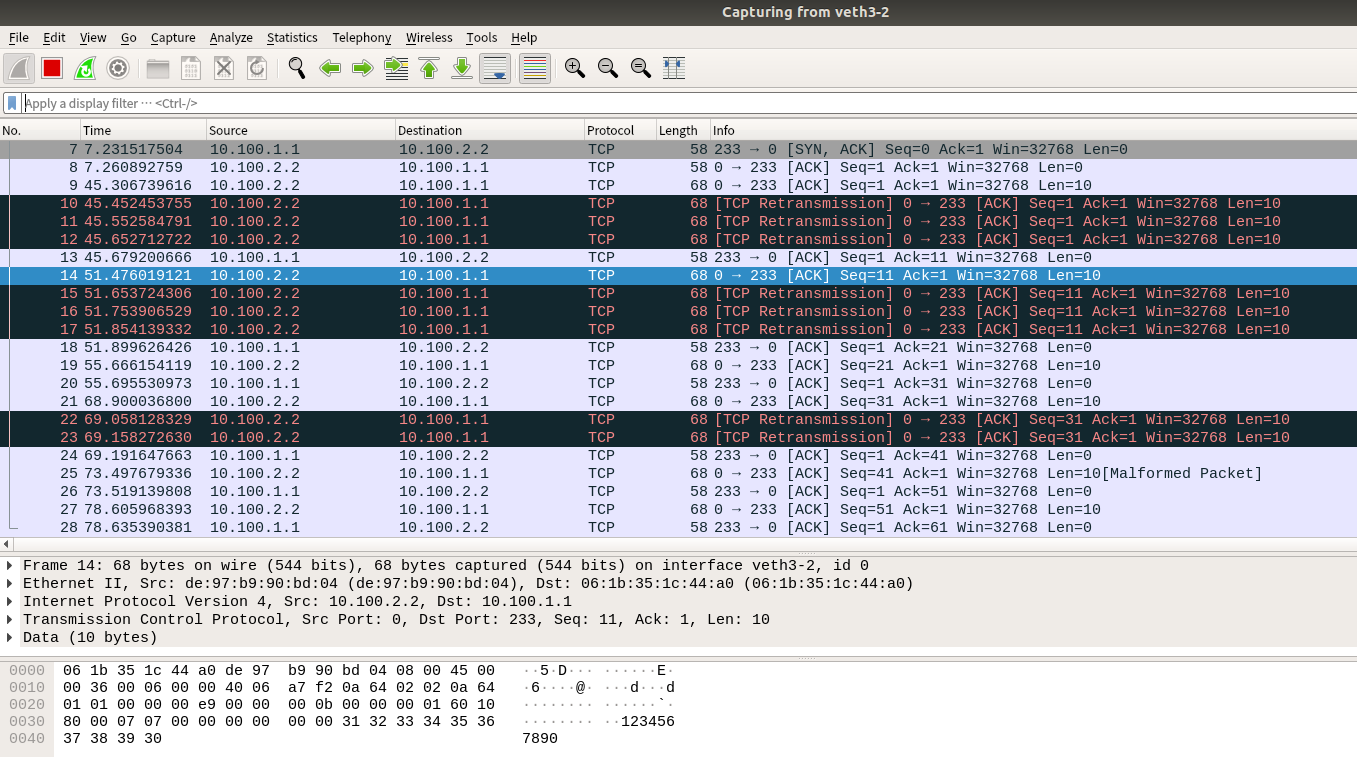
\includegraphics[width=0.9\linewidth]{../lab-netstack-premium-master/checkpoints/CP7.png}
	\caption{CP-7: The frame we send on device \texttt{ns3}}
	\label{fig:CP7}
	\end{figure}
	
	\par The TCP Header locates in bit \texttt{0x0022 $\sim$ 0x39}. and the meaning is shown in the following table.
	
	\begin{itemize}
		\item \texttt{0x0022 $\sim$ 0x0023}: the source port of the connection.
		
		\item \texttt{0x0024 $\sim$ 0x0025}: the destination port of the connection.
		
		
		\item \texttt{0x0026 $\sim$ 0x0029}: sequence number of the segment
		
		
		\item \texttt{0x002a $\sim$ 0x002d}: the acknowlegde number that the source device want to ack. used if \texttt{ACK} bit is on.
		
		\item higher 4 \texttt{0x002e}: the number of long(32 bit) contained in TCP header, $6$ in this packet
		
		\item lower 6 bits \texttt{0x002f}: the control bits, which are \texttt{URG, ACK, PSH, RST, SYN, FIN} from high to low respectively.
		
		\item  \texttt{0x0030 $\sim$ 0x31}: the window size of the prefered receiving packet size if the receiver send message to sender.
		
		\item  \texttt{0x0032 $\sim$ 0x0033}: the checksum of the header, including length and ip address.
		
		\item  \texttt{0x0034 $\sim$ 0x0035}: the urgent pointer, point to the data which is required to process as quick as possible. Used only \texttt{URG} is set.
		
		\item  \texttt{0x0036 $\sim$ 0x0039}: the options in TCP header.
		
		
	\end{itemize}
	
	\subsection*{CP8}
	
	\par Set UP the virtual network saved in \texttt{network1.txt}. and then launch 2 bashs, which located in \texttt{ns1,ns2}. In each bash, launch the server and you can interact with the server.
	
	\par In the below image is my testing trace with server. First I build the connection between two servers, which have the port address \texttt{10.100.1.1:233} and \texttt{10.100.1.2:0}. The I send messages in both direction, and it shows that it can support a Half Duplex communications between servers. 
	
	\par The packet captured in \texttt{veth1-2} at \texttt{ns1} while we testing the communications is provided in \texttt{checkpoints/test1-connection.txt}, which can be load using wireshark. The screen shot of the interact trace can also be found in \texttt{checkpoints}.
	
	\begin{figure}[htbp]
		\centering
		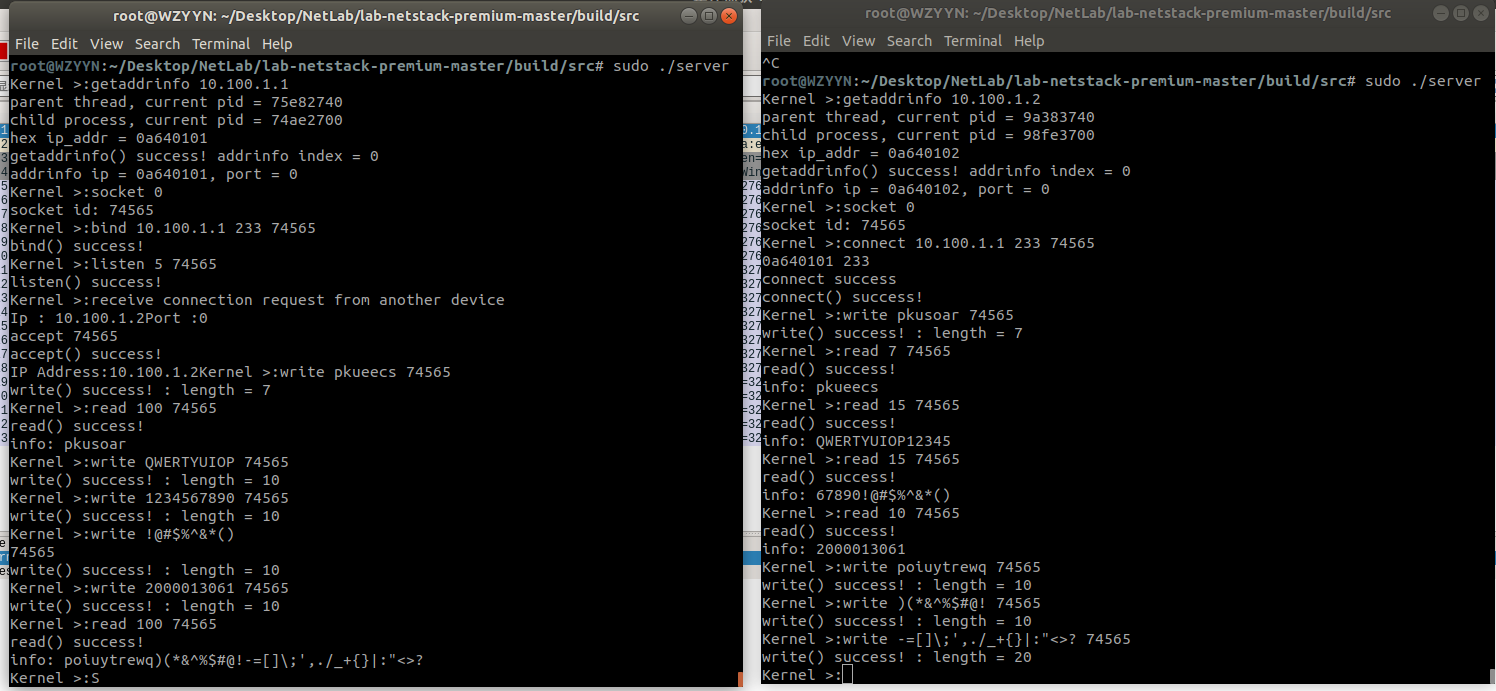
\includegraphics[width=0.9\linewidth]{../lab-netstack-premium-master/checkpoints/test1-connection.png}
		\caption{CP8-1: the connection is currectly set up.}
		\label{fig:CP8-1}
	\end{figure}
	
	\par If we set packet drop using \texttt{tc qdisc add dev veth2-1 root netem loss 50\%} in \texttt{ns2} after the connection is set up, Then the server can correctly detect the packet loss if the message is not acknowledged. After the packet loss is set up, I send 7 different messages from \texttt{ns1} to \texttt{ns2}; one of them have exactly \texttt{1} retransmission, and the other one have \texttt{3} retransmission. The screen shot of the interact is shown below and the packet captured in \texttt{veth2-1} is provided in \texttt{checkpoints/test2-retransmission.txt}
	
	\begin{figure}[htbp]
		\centering
		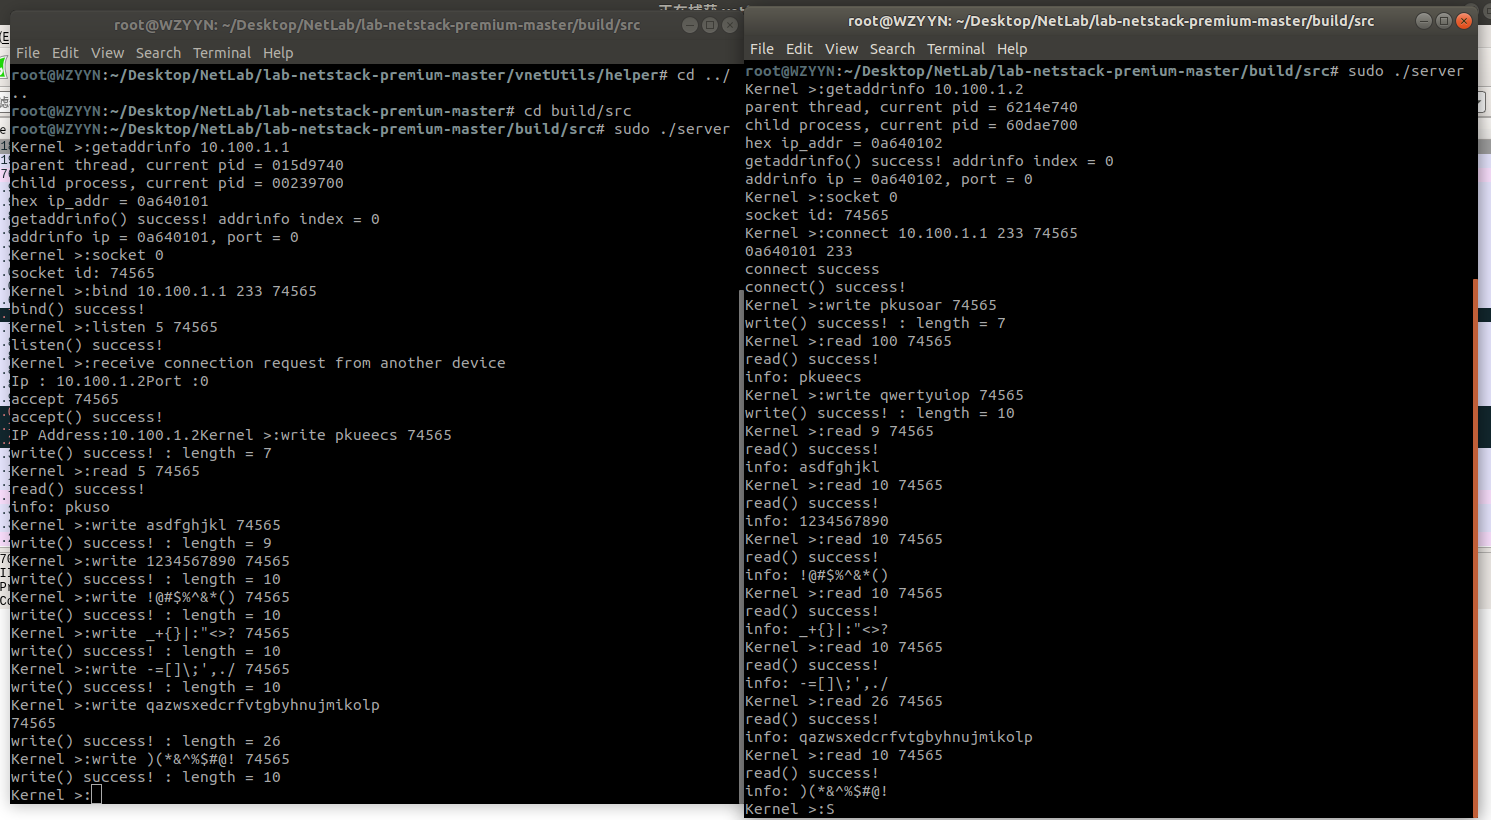
\includegraphics[width=0.9\linewidth]{../lab-netstack-premium-master/checkpoints/test2-retransmission.png}
		\caption{CP8-2: retransmit the message if ACK is blocked.}
		\label{fig:CP8-2}
	\end{figure}
	
	\par Also I test is the message is blocked. I run \texttt{server} in \texttt{ns1,ns3}, and \texttt{router} in \texttt{ns2}. After connection is set up, I use \texttt{tc qdisc add dev veth2-1 root netem loss 50\%} to set packet drop, and send $6$ different message to \texttt{ns1}. Almost every one have retransmission happened, and they are received by \texttt{ns1} in correct order. The screen shot of the interact is shown below and the packet captured in \texttt{veth3-2} is provided in \texttt{checkpoints/test3-retransmission.txt}
	
	\begin{figure}[htbp]
		\centering
		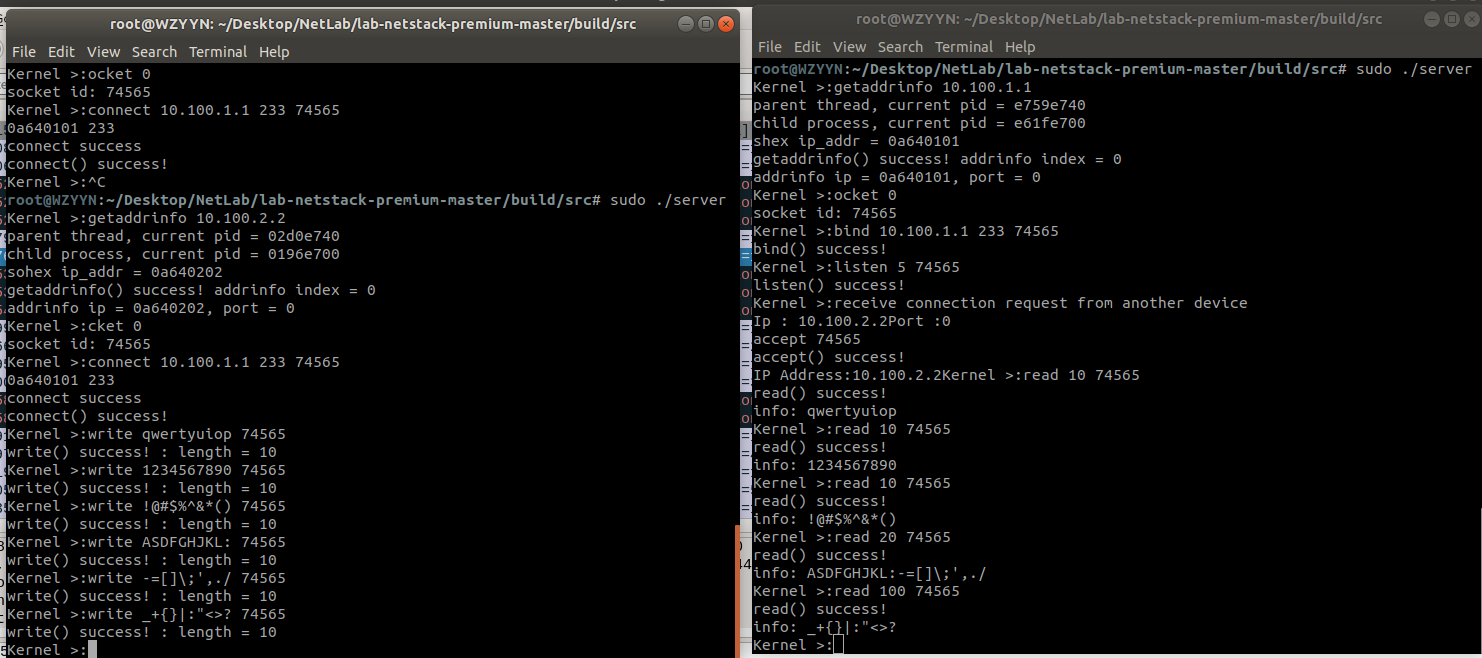
\includegraphics[width=0.9\linewidth]{../lab-netstack-premium-master/checkpoints/test3-retransmission.png}
		\caption{CP8-3: retransmit the message if message is blocked.}
		\label{fig:CP8-3}
	\end{figure}
	
	
	
	
		
\end{document}